\documentclass[11pt]{article}
\usepackage[margin=1in]{geometry}

\usepackage{amsmath}
\usepackage{amssymb}
\usepackage{physics}
\usepackage{graphicx}

\usepackage{hyperref}

\renewcommand{\d}[2][]{\mathrm{d}^{#1}{#2}}



\begin{document}


\section{Introduction}


\section{TDA}
For any discrete data set, persistent homology entails a sequence of simplicial complexes ($\alpha$, Vietoris-Rips, \&c.) of varying granularity in which homological cycles first appear and then disappear. The choice in filtration corresponds to different ways to add edges and faces to the simplicial complex as some parameter is varied. This process produces a collection of persistence data consisting of births and deaths, $\{b_i,d_i\}$, for each of the cycles. Persistence diagrams are a way to visualize these topolgically derived data.

The persistence diagram contains information about the size of features in the data. Since such topological data are robust against small perturbations in the original data set, TDA is a useful tool in statistical analyses of many systems.


(Why persistence image is necessary... robustness against sudden appearence of cycles, small perturbations in persistence data, \&c.) To create the persistence image, begin by transforming the persistence data to $\{b_i,p_i\}=\{b_i,d_i-b_i\}$. Each point is then smoothed, which allows for small perturbations in the topological data to have small effects. Choosing gaussians of fixed width, the full density is
\begin{align}
    \rho(x,y) &= \sum_i w(b_i,p_i)\;\frac{1}{2\pi\sigma^2}\exp\left[-\frac{(x-b_i)^2+(y-p_i)^2}{2\sigma^2}\right]
\end{align}
The weighting function should be chosen so that $w(b_i,0)=0$; this ensures that the sudden appearence of a cycle is accounted for smoothly (choice here?). The persistence image is then the vector obtained by integrating $\rho$ over a series of ``pixels'' (bins):
\begin{align}
    I_\text{p} &= \iint\limits_\text{p}\rho(x,y)\,\d{x}\d{y}
\end{align}
This process can be done for $H_0,H_1,\ldots$ and the respective vectors adjoined or treated separately. Ultimately, we have now a vector in $\mathbb{R}^n$ ($n$ not too large!) which is a representation of the homological structure of the original data set.

\begin{figure}[b]
    \centering
    \includegraphics[]{}
    \caption{Example PD$\rightarrow\rho\rightarrow$PI process.}
\end{figure}



\section{Spin Models}
Here we will apply the techniques of TDA to lattice spin systems. The traditional Ising model is rich in behaviour, despite being simple to describe; in two or more dimensions there is a second-order phase transition from an ordered to random state. While it is relatively easy to distinguish between these states simply by looking at the spin configurations, there exists systems in which the different states are not as readily identified. It has been demonstrated that one can use machine learning to identify phases of matter for such spin systems. We will show that this classification can also be done using persistance images built from the spin configurations, where physical characteristics of the data such as sizes of features play a central role.

As a starting point we begin with the 2d Ising model on a square lattice:
\begin{equation}
    \beta H = \sum_{\langle ij\rangle}s_is_j + h\sum_is_i
\end{equation}
where the sum is over all pairs of adjacent spins (check normalization). Each $s_i$ takes values in $\{-1,1\}$. We will be interested in the case of no external magnetic field, $h=0$.

\begin{figure}[t]
    \centering
    \includegraphics[]{}
    \caption{Example spin configurations above and below phase transition.}
\end{figure}

We take as data the physical locations of spins which all point in the same direction as the majority of spins after reaching equilibrium with a thermal bath. At very low temperatures when nearly all spins are aligned cycles are born and die very quickly, while at high temperatures features in the spins may be longer-lived.


Of interest also are spin systems in which there are topological phases, such as the $\mathbb{Z}_2$-gauged Ising model (see [\textit{Gauge fields...}, Balian et.al.]). These theories enjoy a local gauge invariance which ensures that there is spontaneous magnitization at low temperatures. Rather, in dimensions $d>2$ the phase transition is signalled by a change in the spin-spin correlation function. For $C$ a closed path in the lattice, at low temperature one finds a ``perimeter law",
\begin{equation}
    \langle\prod_C s_i\rangle \sim e^{-h(\beta)L}
\end{equation}
while at high temperatures one finds an ``area law",
\begin{equation}
    \langle\prod_C s_i\rangle \sim e^{-f(\beta)A}
\end{equation}
for $L$ the length of the path $C$ and $A$ the minimum number of plaquettes needed to span $C$. The arguments which lead to these expressions do not apply in $d=2$ (see section V.D.~of [\textit{An introduction...}, Kogut]) as the radius of convergence for the validity of the perimeter law is zero. One may also understand the special case of $d=2$ as being a consequence of the equivalence
\begin{equation}
    \Big(\text{2d }\mathbb{Z}_2\text{-gauged Ising model}\Big) = \Big( \text{1d Ising model} \Big)
\end{equation}
found by comparing the partition functions of the two models after having chosen a convenient gauge. One can, however, still hope to distinguish between high and low temperature spin configurations, as correlation lengths do change with temperature.

For $d>2$ we can hope to do more: not only identify high and low temperature configuration but also determine the critical temperature at which one shifts from a perimeter to area law. All of this occurs without the obvious spontaneous magnitization that is present in the 2d Ising model. (We will see if...) TDA techniques are powerful enough to pick up on this distinction in the topolocial ordering of the states.

\subsection{Ising Model}
Spins sit at vertices of cubical lattice.
\begin{equation}
    H = -\sum_{\langle i,j\rangle}s_is_j
\end{equation}
Sum is over all pairs of adjacent spins.

Energy per spin should be $-d$ at $T=0$ and 0 at $T=\infty$.

\begin{itemize}
    \item 2d: Phase transition at $T_\text{c}\approx 2.269$ from ordered to disordered.
    \item 3d: Phase transition at $T_\text{c}\approx 4.512$ from ordered to disordered. Finite $N$: $T_\text{c}^{-1}\approx 0.2212-\frac{2.4454}{N}$ (see [0406135]).
\end{itemize}

\begin{figure}[h]
    \centering
    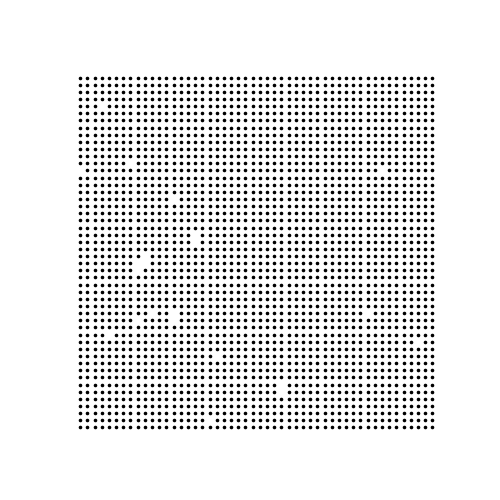
\includegraphics[width=0.3\textwidth]{ising_T=150.png}
    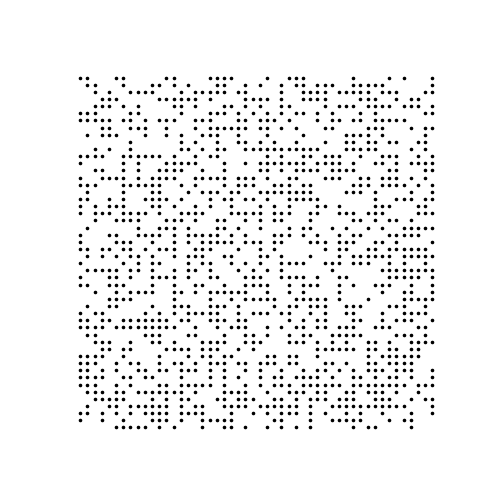
\includegraphics[width=0.3\textwidth]{ising_T=inf.png}
    \caption{Example configurations for Ising model at $T=1.5$ (left) and $T=\infty$ (right).}
\end{figure}

\subsection{Square Ice Model}
Spins sit on edges of cubical lattice.
\begin{equation}
    H = \sum_v\Big(\sum_{i\in v}s_i\Big)^2
\end{equation}
$v$ are the vertices and $i\in v$ is a sum over spins on edges connected to that vertex.

Energy per spin should be 0 at $T=0$ and 2 at $T=\infty$.

\begin{itemize}
    \item 2d \& 3d: Based on $\ev{E}$, phase transitions somewhere around $T=1\to2$.
\end{itemize}

\begin{figure}[h]
    \centering
    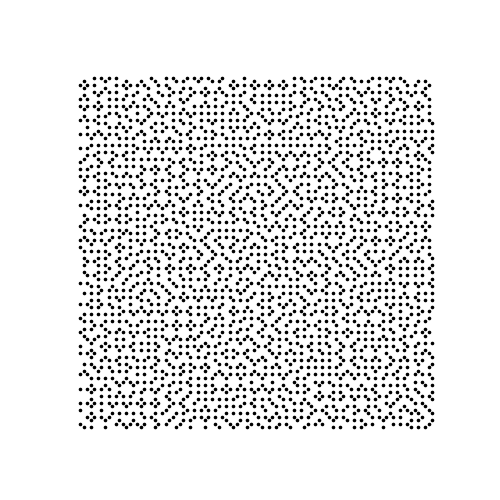
\includegraphics[width=0.3\textwidth]{squareice_T=0.png}
    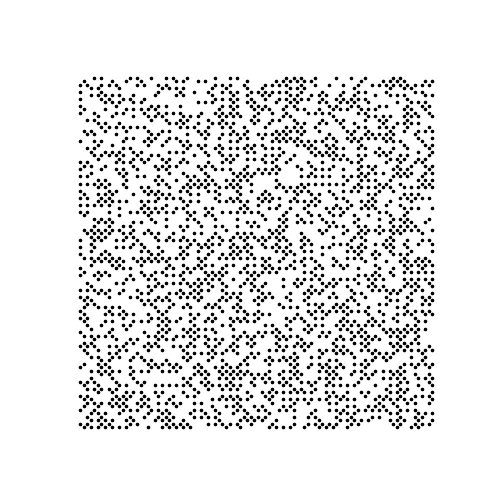
\includegraphics[width=0.3\textwidth]{squareice_T=inf.png}
    \caption{Example configurations for square ice model at $T=0$ (left) and $T=\infty$ (right).}
\end{figure}


\subsection{$\mathbb{Z}_2$-gauge Ising Model}
Spins sit on edges of cubical lattice.
\begin{equation}
    H = -\sum_p\prod_{i\in p}s_i
\end{equation}
$p$ are the ``plaquettes'' and $i\in p$ is a product over spins around the face.

Energy per spin should be $\frac{1-d}{2}$ at $T=0$ ($dN^d$ spins and $\binom{d}{2}N^d$ plaquettes) and 0 at $T=\infty$.

\begin{itemize}
    \item 2d: No phase transition. Can still hope to classify $T=0$ vs $T=\infty$.
    \item 3d: No spontaneous magnetization. Phase transition at $T_\text{c}\approx??$ from perimeter- to area-law correlation functions. (Couldn't find value in lit... judging from $\ev{E}$ seems to be around 1.)
\end{itemize}

\begin{figure}[h]
    \centering
    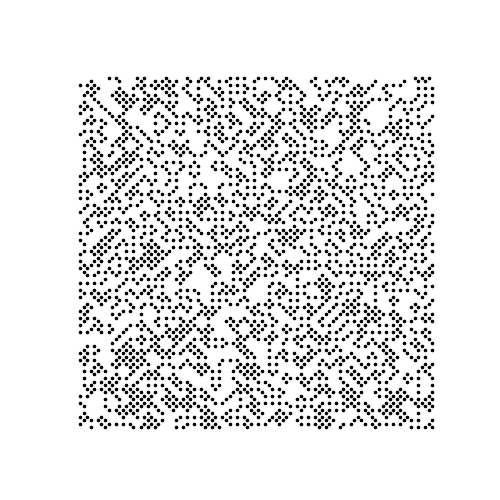
\includegraphics[width=0.3\textwidth]{gauged_T=0.png}
    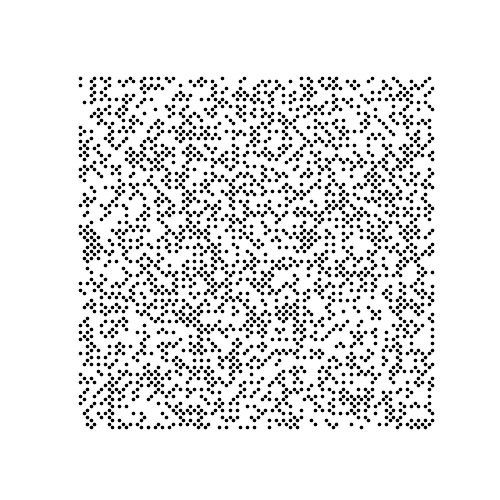
\includegraphics[width=0.3\textwidth]{gauged_T=inf.png}
    \caption{Example configurations for gauged Ising model at $T=0$ (left) and $T=\infty$ (right).}
\end{figure}


\section{Results}
\begin{itemize}
    \item Choices in data collections
    \item Classification with different methods (logreg, kmeans, PCA, \&c.)
    \item Estimation of critical temperature from unsupervised learning methods
\end{itemize}

2d Ising: Wolff cluster algorithm, average of $20$ flips per spin, $T\in\{1.00,1.05,1.10,\ldots,3.50\}$, 500 at each temperature.


(TO DO:) Near $T_\text{c}$ we expect the characteristic scale-invariance of critical phenomena to be evident in the persistance diagrams/images. By considering temperatures close to $T_\text{c}$ we hope to find signatures of the diverging correlation length in the derived topological data.


\section{Discussion}


\end{document}